\chapter{Multi-Cell System Performance Analysis under Correlated Shadow Fading}\label{ch:Multi}
\par In a cellular network, connections between the Base Station (BS) and Mobile Users (MUs) may fail when the channel is in deep fade. Shadow fading is large-scale fading which can cause significant received power loss for a wide area. Correlated shadow fading will result in correlated long outage durations. Power outage will lead to connection loss and/or packet loss which is harmful to MUs, especially to those who are using real-time applications such as video conferencing. Intuitively, increasing BS density is considered to be an efficient way to reduce outage and provide better Quality of Service (QoS) support for delay sensitive applications in noise-limited regime. This chapter is an extension of Chapter \ref{ch:ExpSingleCell}, which focuses on a study of the performance of a multi-cell communication system under correlated shadow fading. We consider the downlink direction in a multi-cell communication system. To investigate the outage probability given correlated shadow fading and different BS densities, two system layouts, Grid model and Random model, are studied. First, we compare the outage probability with same correlated shadow fading with regard to the two different system layout. Grid layout performs better than Random layout. Secondly, we compare the outage probability with independent shadow fading and with the correlated shadow fading for Random model. The received signal-to-interference-plus-noise ratio (SINR) is calculated by assuming independently Gaussian and jointly Gaussian shadow fading at the MU. Thirdly, we focused on Random model which is more realistic and compared the outage duration under two circumstances: independent shadow fading and correlated shadow fading. Simulation results show that the outage durations with correlated shadow fading are longer than that of the independent shadow fading. At last, we showed that increasing BS density can reduce the effect of correlated shadow fading and improve the system performance in terms of outage probability and outage duration. 
\section{Background}
\par In a cellular communication system, the connection between the BS and a MU may be dropped when the user enters a deeply shadowed area. Fading phenomena can substantially affect the performance of a wireless communication system. In general, fading can be divided into two categories: large-scale fading and small-scale fading. A signal transmitted from source to destination will experience both large-scale and small-scale fading. Small-scale fading is caused by multipath propagation. Large-scale fading, which is also known as shadow fading, is caused by obstacles (trees, buildings, etc.) in the propagation path. In most cases, shadow fading is assumed to be temporally and spatially independent \cite{rappaport1996wireless}.  Researchers have also shown that shadow fading is spatially correlated at different positions on the propagation path \cite{gudmundson1991correlation}, \cite{zhang2008novel}. In \cite{fabbri2009impact} and \cite{patwari2008effects}, the effects of correlated shadowing in connectivity is demonstrated, which indicates that reliable connectivity will be much more difficult to maintain than indicated by independent shadow fading models. The spatial correlation of shadow fading is important when studying the quality of service of a mobile system since it will result in long-lasting outage durations, which will deteriorate the performance of the applications running on the network. The focus of this chapter is to study channel variations and system performance due to correlated shadow fading in a multi-cell communication system and provide a solution to reduce the frequency and duration of dropped connections and improve system performance by increasing BS density.
\par There have been a lot of studies on the outage probability of cellular communication systems \cite{abu1991outage, petrovic2013outage, emamian2014outage}. The author of \cite{vural2015effect} analyzed the outage probability and coverage area under different independent identical distributed (i.i.d.) shadow fading distributions: Log-normal distribution, Weibull distribution and Gamma distribution. In contrast, there is much less work on the outage probability and outage duration given correlated shadow fading. The system performance of multi-cell system given correlated shadow fading is still an open problem. In \cite{lu2015long} and \cite{lu2015shining} we studied the outage probability and outage duration of a single cell communication system under exponentially correlated shadow fading and Distance-Angle correlated shadow fading. \cite{lu2015long} we showed that for a single cell model, exponentially correlated shadow fading can be modeled as a Markov Chain Model. Highly correlated shadow fading will result in long-lasting outage durations. In \cite{lu2015shining}, single cell given distance-angle correlated shadow fading system is studied. The correlated shadow fading also lead to correlated outage and long outage durations in a single cell model. In this case, we provide a solution to overcome the correlated shadow fading: relay cooperative communication. Chapter \ref{ch:CoopComm} and Chapter \ref{ch:ExpSingleCell} are limited to single-cell model. In this chapter, we are going to extend the study of correlated shadow fading impact to a multi-cell communication system, and provide a solution to overcome the long-lasting outage duration.
\par For multiple-cell system, in \cite{andrews2011tractable}, the author develop new general models for the multi-cell signal-to-interference-plus-noise ratio (SINR) using stochastic geometry. The cellular networks is modeled by placing the BSs at locations as a homogeneous Poisson Point Process. The author concluded that under general fading, increasing the number of BSs does not affect the coverage probability (so is the outage probability) while the MU is connected to the nearest BS. The paper also did comparison between grid model and the random PPP model and concluded that a regular grid provided the upper bound of the coverage probability while the PPP provided the lower bound. The author also considered the effect on independent log-normal interference and concludes that the increasing log-normal interference increased the coverage probability which seems counter-intuitive. In this paper, the author didn't consider the scenarios with correlated log-normal interference. Only the coverage probability is studied, analysis of outage duration is not analyzed. 
\par A comparative study of random and grid topology of small cell network deployment was given in \cite{chen2012small}. In this paper, spatial outage probability and spatial average throughput versus the number of access points of the two different network deployment is studied. But this paper considered independent log-normal interference instead of correlated log-normal fading. Approximate outage probability and capacity for $\kappa-\mu$ shadow fading is studied in \cite{kumar2015approximate}. $\kappa-\mu$ shadow fading includes one-side Gaussian, the Rayleigh, the Nakagami-m, the Rician. As we mentioned before, the imperial measurements didn't exhibit such complicated features of shadow fading. So comparing with correlation, those complex features are not of main focus.
\par As we have mentioned in previous chapters, in most cases shadow fading is modeled as an independent log-normal distribution. But this model fails to capture the spatial correlations in shadow fading. This chapter contains three major sections: first part describes the correlated shadow fading model that was used and the resulting correlated outage field; second part studies the outage probability given Grid layout and Random layout; third part investigates the outage probability and outage duration of the system given different BS densities, different correlation parameters and different connection strategies. The key contributions of this chapter are summarized below.
\begin{itemize}
\item Correlated outage fields are given to analyze the relationship between correlated shadow fading and correlated outage events. 
\item Investigate outage probability analysis of both Grid layout and Random layout.
\item Show how increasing BS densities help mitigate correlated shadow fading in Random layout in terms of outage probability (coverage probability) and outage durations.
\item Analyze the relation between the tunable parameter of the correlated shadow fading model and the outage probabilities.
\item Compare the system performance of different MU-BS connection strategies: MU connecting to the nearest BS and MU connecting to the BS providing strongest signal.
\end{itemize}
The chapter is organized as follows: Section \ref{CorrShadowField} presents the correlated shadow fading model that is used in this paper and the resultant correlated outage field. Section \ref{SystemModel} presents the system model with two different BS deployment schemas and investigates the outage probability given different BS layout. Section \ref{OutageProb} gives theoretical analysis of outage probability given correlated shadow fading. Section \ref{SimuProb} presents the simulation setup and analyzes the simulation results of different BS deployments and densities. Section \ref{ch4:conclusion} summerizes the chapter and proposes future work directions.
\section{Correlated Shadow Fading}
\label{CorrShadowField}
As stated in the background, empirical measurements show that there exist different patterns of correlations between the shadowing. The independent log-normal shadow fading model, while very useful for static MS performance analysis, cannot reflect the correlation of shadow fading between different locations. In this section, we will give a brief introduction of shadow fading models, including the model used in this chapter.
There is no single mathematical model which captures all different categories of correlation\cite{szyszkowicz2010feasibility}. In Chapter \ref{ch:CoopComm}, a distance-angle correlation model is used and in Chapter \ref{ch:ExpSingleCell} an exponential correlation model is used. The correlation matrix of angle-distance model is given below:
\begin{equation}
\mathbf{K}_{N\times N} = [ \sigma_{s}(\vec{r_{i}})\sigma_{s}(\vec{r_{j}})h(\vec{r_{i}}\vec{r_{j}})],
\label{correlationmatrix}
\end{equation}
where $N$ paths interfere with path $\vec{r_{i}}$ and $\mathbf{E}\{S_{i}^{2}|\vec{r_{i}}\}=\sigma_{s}^{2}(\vec{r_{i}})$. This model assumes that in the correlation matrix, $h$ is separable with respect to the angle of arrival
\begin{equation}
\theta = |\angle\vec{r_{i}}-\angle\vec{r_{j}}|\in [0^{\circ},180^{\circ}],
\end{equation}
and the arrival distance ratio
\begin{equation}
R=|10\log_{10}r_{i}/r_{j}|=\frac{10}{\ln 10}|\ln r_{i}-\ln r_{j}|,
\end{equation}
\begin{equation}
h(\vec{r_{i}},\vec{r_{j}})=max\{1-\theta/\theta_{0},0\}\cdot max\{1-R/R_{0},0\}.
\end{equation}
The correlation coefficients is a piece-wise linear function of the angle of arrival and the arrival distance ratio. Due to this feature, when cell size decreases (BS density increases), the correlation between two points also decreases. This violate the physical characteristic of shadow fading. The size of obstacle which causes the shadow fading does not change when the cell size changes, therefore the correlation between two different position should not change when cell size changes. As stated above, the angle-distance model is not suitable for analyzing mulit-cell system performance. In this chapter, we use the exponentially correlated shadow fading model \cite{szyszkowicz2011interference} the same as in Chapter \ref{ch:ExpSingleCell}. In \cite{szyszkowicz2011interference}, the author states that correlation in shadowing is indispensable for the analysis of interference of large networks. An exponentially correlated shadowing field $S$ with shadow fading factor $s_{i}$ for each position $p_{i}$ has a correlation matrix as below:
\begin{equation}
\mathbf{K}_{N\times N} = [ \sigma_{s}(p_{i})\sigma_{s}(p_{j})\rho(i,j)],
\label{correlationmatrix}
\end{equation}
where $N$ is the length of the shadowing field. Suppose $A$ and $B$ are two neighbouring points, the shadow fading (in dB) is $N(0,\sigma^2)$ where $\sigma$ is the standard deviation. The spatial correlation between $s_{A}$ and $s_{B}$ will be given by 
\begin{equation}
\rho_{A,B} = \frac{E[s_{A}s_{B}]}{\sigma^2} =e^{-\frac{d_{A,B}}{d_{0}}}
\end{equation}
\begin{figure}
\centering
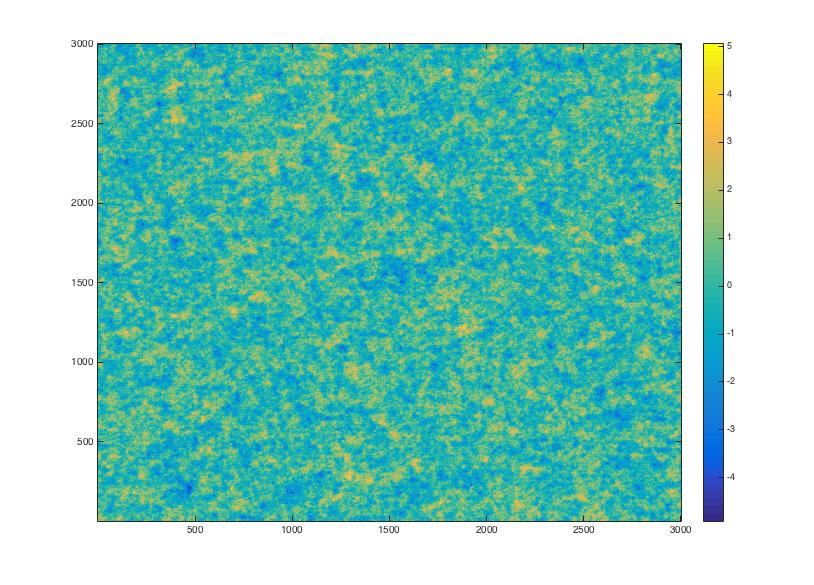
\includegraphics[width = 10cm]{ShadowFieldDeCorr20.jpg}
\caption{Exponentially correlated shadowing field with $d_{0} = 20m$ (the color of the area refers to the normalized standard deviation which is $S_{i}/\sigma_{s}(i)$)}

\label{ch4:shadowingfield}
\end{figure}

Following the shadowing field generation algorithm, we generate shadowing fields with different values of de-correlation distances. A sample shadowing field is shown in Figure \ref{ch4:shadowingfield}.
\par Let $\varphi = \{1, 2, \dots, N\}$ denotes the set of all Base Stations, then the received signal from Base Station $j$ to the destination user $D$ is given by:
\begin{equation}
y_{i\to D} = G_{i\to D}x_{i}+n_{D}.
\end{equation}
where $x_{i}$ is the signal transmitted by the source Base Station and $y_{i\to D}$ is the signal received by the destination. $n_{D}\sim \mathcal{CN}(0,N_{0})$ is additive white Gaussian noise. $G_{i\to D}$ is the channel gain from source Base Station to destination including path loss and shadow fading. The end-to-end received signal-to-interference-plus-noise ratio $\text{SINR}$ is given as follows:
\begin{equation}
\text{SINR} \triangleq \frac{P_{i}*G_{i\to D}^{2}}{N_{0}+\sum_{j\in \varphi/i}P_{j}*G_{j\to D}^2},
\end{equation}
where $P_{i}$ is the transmitted power of Base Station $i$. The destination successfully receives the signals if no outage event happens, i.e., $\log_{2}(1+\text{SINR})\ge R$, where $R$ is the required data rate. From the definition of SINR, no outage event happens as long as $\text{SINR} > \gamma$, where $\gamma = 2^{R}-1$.
\par Given a correlated shadowing field, the outage events at different locations are also correlated. Without considering other small-scale fading, the channel gain at different locations has a spatial correlation. Given a proper threshold $\gamma$, an outage area is defined as channel gain less than $\gamma$. Based on the aforementioned correlated shadow fading model and Random system model, a correlated outage filed can be generated as in Figure \ref{outagefie}. On the left, a correlated outage field with independent log-normal shadow fading is shown while the correlated outage field with correlated shadow fading is given on the right. The black color indicates outage areas. Outage area with i.i.d. shadow fading are nonconsecutive dots while with correlated fading are connected areas. This demonstrates correlated outage areas come with correlated shadow fading.

\begin{figure*}
\centering
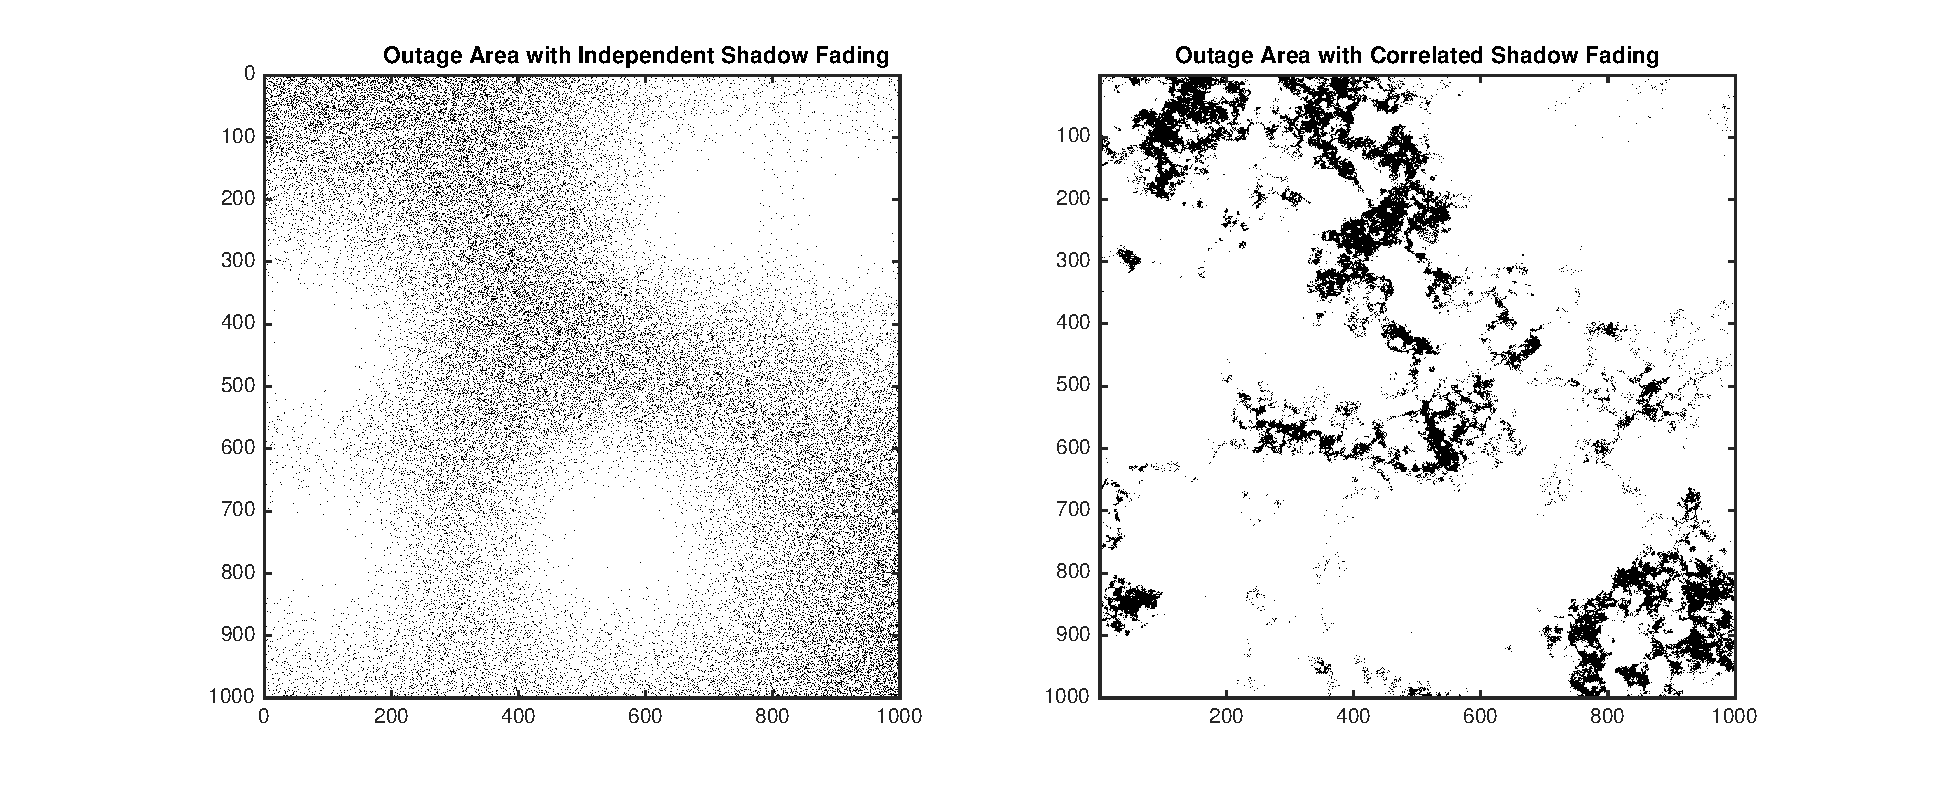
\includegraphics[width=14cm]{outageArea.eps}
\caption{Correlated Outage Fields with $\gamma$ (Dark areas are outage areas while white areas are non-outage areas)}
\label{outagefie}
\end{figure*}
\section{System Model}
\label{SystemModel}
In this paper, we considered two system models with two different BS deployment scheme: Grid model and Random model.
\begin{itemize}
\item Grid Model: $\lambda$ BSs are placed on a regular grid deterministically.
\item Random Model: $\lambda$ BSs are placed randomly in a fixed area.
\end{itemize}
\begin{figure}
\centering
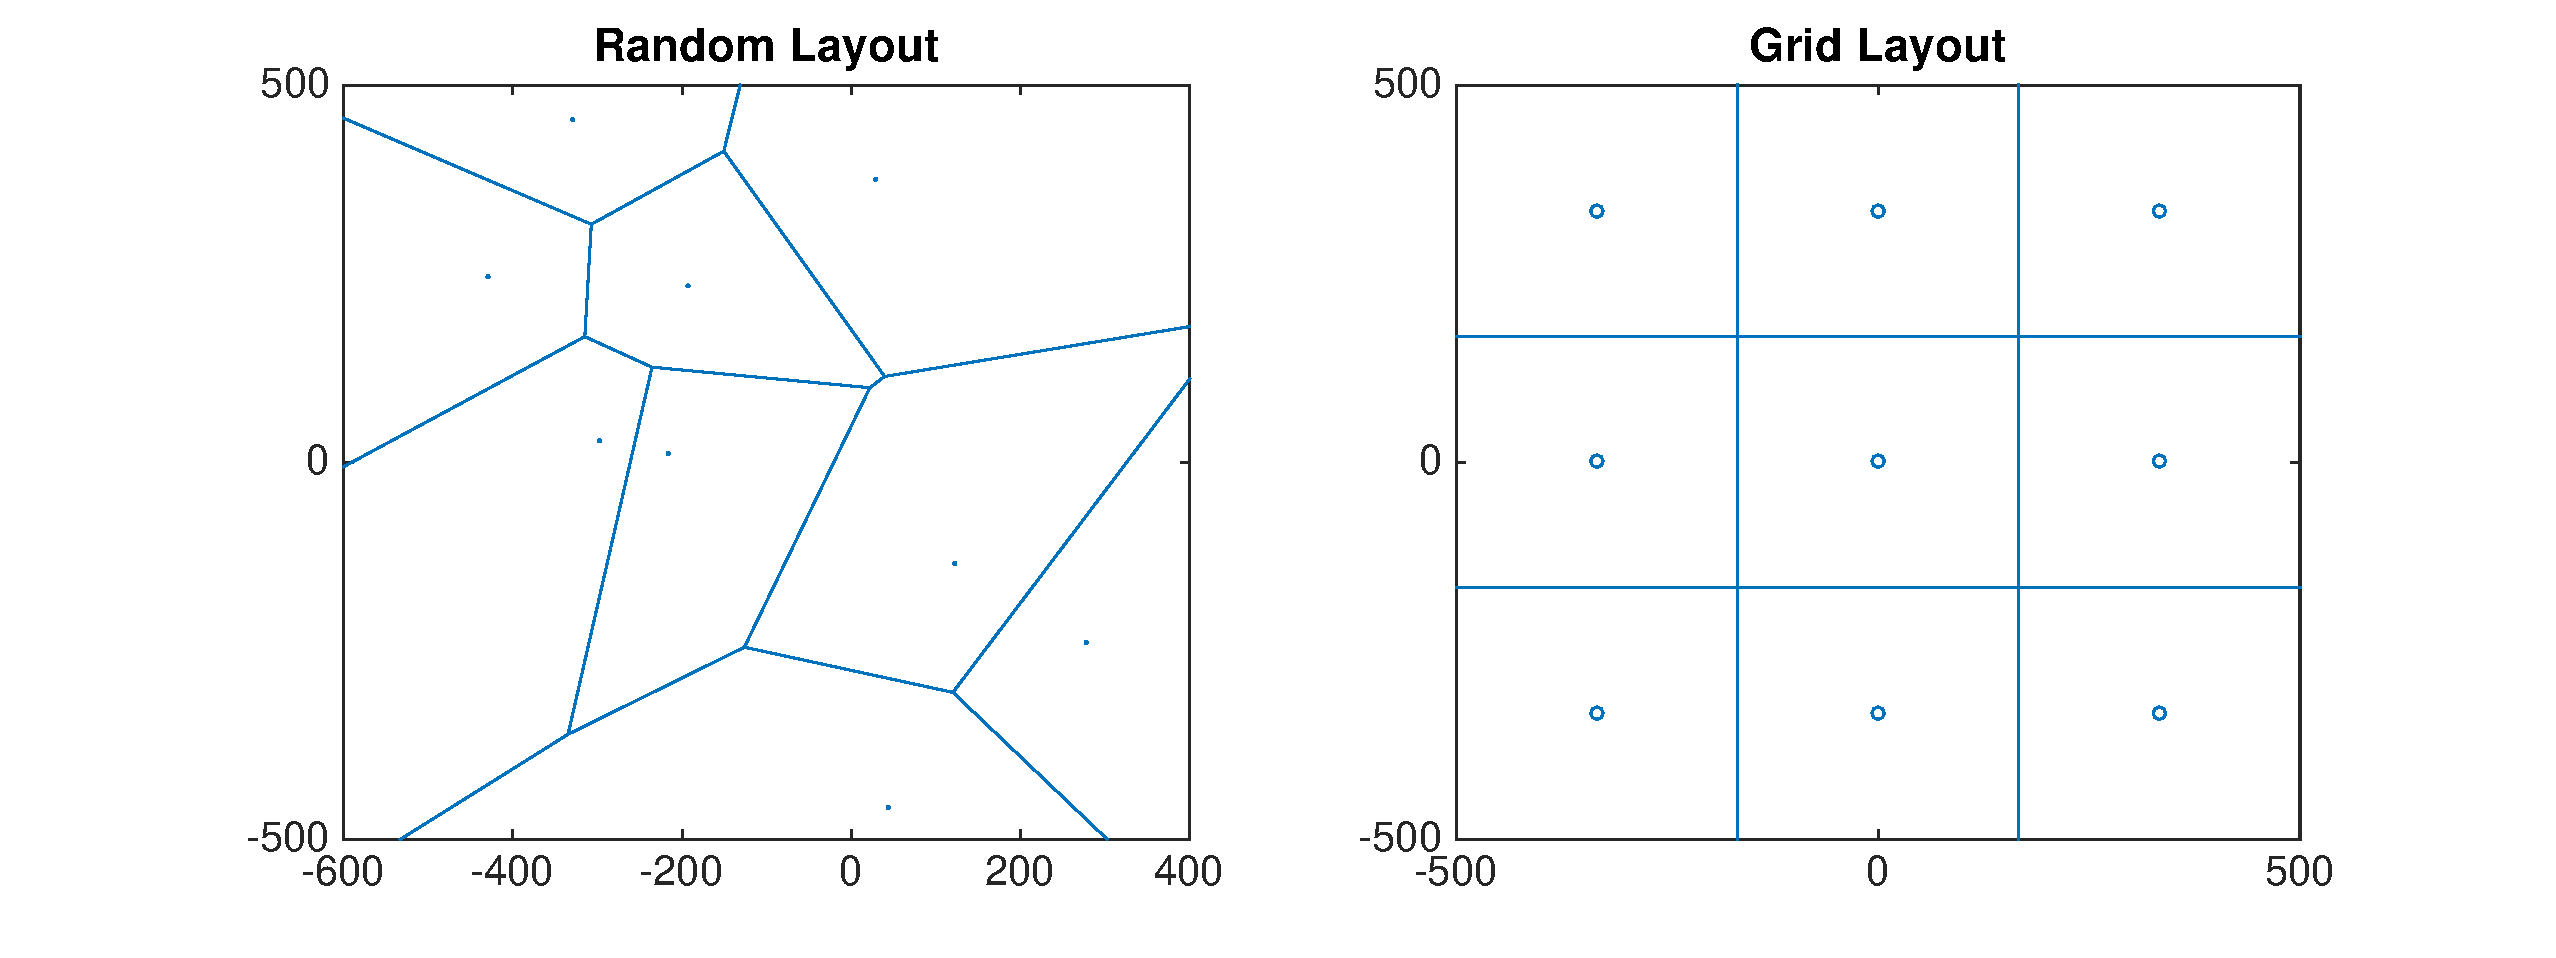
\includegraphics[width=14cm]{systemLayout.eps}
\caption{Random Layout and Grid Layout with $\lambda = 9$.}
\label{RandomLayout}
\end{figure}
% \begin{figure}
% \centering
% \includegraphics[width=8cm]{GridLayout.eps}
% \caption{Grid Base Station Locations}
% \label{GridLayout}
% \end{figure}
Left figure of Fig \ref{RandomLayout} is an example of the traditional grid model, where cells are in regular square shape with same size. For the Random model showed in Fig \ref{RandomLayout} right subfigure, cells are not guaranteed to be the same shape and same size. Nearest distances between different cells are in a large variation. 
\section{Outage Probability Analysis}
\par Let $\varphi = \{1, 2, \dots, N\}$ denotes the set of all Base Stations, then the received signal from Base Station $j$ to the destination user $D$ is given by:
\begin{equation}
y_{i\to D} = G_{i\to D}x_{i}+n_{D}.
\end{equation}
where $x_{i}$ is the signal transmitted by the source Base Station and $y_{i\to D}$ is the signal received by the destination. $n_{D}\sim \mathcal{CN}(0,N_{0})$ is additive white Gaussian noise. $G_{i\to D}$ is the channel gain from source Base Station to destination including path loss and shadow fading. The end-to-end received signal-to-interference-plus-noise ratio $\text{SINR}$ is given as follows:
\begin{equation}
\text{SINR} \triangleq \frac{P_{i}*G_{i\to D}^{2}}{N_{0}+\sum_{j\in \varphi/i}P_{j}*G_{j\to D}^2},
\end{equation}
where $P_{i}$ is the transmitted power of Base Station $i$. The destination successfully receives the signals if no outage event happens, i.e., $\log_{2}(1+\text{SINR})\ge R$, where $R$ is the required data rate. From the definition of SINR, no outage event happens as long as $\text{SINR} > \gamma$, where $\gamma = 2^{R}-1$.
\par Given a correlated shadowing field, the outage events at different locations are also correlated. Without considering other small-scale fading, the channel gain at different locations has a spatial correlation. Given a proper threshold $\gamma$, an outage area is defined as channel gain less than $\gamma$. 
\par For a particular MU, outage happens when its received SINR is less than a threshold to decode the received signal. In our scenario, the probability that the receiver cannot decode signals received from its serving Base Station is defined as:
\begin{equation}
P(out_{i}) = P[\text{SINR}_{i\to D} < \gamma],
\end{equation}
We investigate two connection strategies: MU connect to the nearest BS and MU connect to the BS provides strongest signal. If we assume that the user is served by the nearest Base Station, then the outage probability will be $P_{out} = P_{out_{i}}$ where $i$ is the index of the nearest Base Station. Otherwise, the indices of all Base Stations which are able to provide successfully connection to the Mobile User form a set $\mathcal{R}_{n}$. Under the assumption that an MS always connecting to the Base Station which provides the best received signal, the outage event happens if no Base Station can provide big enough SINR to the receiver, which means $\mathcal{R}_{0}=\phi$. Based on this assumption we have:
\begin{equation}
P_{out} = \max_{i = 1,\cdots,N} P[\text{SINR}_{i\to D}<\gamma].
\end{equation}
The probability density function (pdf) of shadow fading $S$ given $L$ correlated fading branches is
\begin{equation}
\begin{split}
f_{\mathbf{S}}(\mathbf{s}) = &\frac{\lambda^{L}}{\sqrt{2\pi}|\mathbf{K}_{L\times L}|^{1/2}\prod_{i=1}^{L}s_{i}}\\
&\cdot\exp(-\frac{1}{2}(10\log_{10}\mathbf{s}-\boldsymbol{\mu})^{T}\mathbf{K}_{L\times L}^{-1}(10\log_{10}\mathbf{s}-\boldsymbol{\mu})),
\end{split}
\end{equation}
where $\lambda = 10/\ln10$ and $\boldsymbol{\mu}$ is the average shadow fading which is normally $0$. $\mathbf{K}_{L\times L}$ is the correlation matrix which is defined in \eqref{correlationmatrix}. Let $\theta_{i} = \frac{10\log_{10}s_{i}-\mu_{i}}{\sqrt{2}\sigma_{i}}$, and doing a change of variables gives us the pdf of $\mathbf{\Theta}$ as follows:
\begin{equation}
f_{\mathbf{\Theta}}(\mathbf{\theta}) = \frac{1}{\pi^(L/2)|\mathbf{\Sigma}|^{1/2}}\exp(-\mathbf{\Theta}^{T}\mathbf{\Sigma}^{-1}\mathbf{\Theta}),
\end{equation}
where $\mathbf{\Sigma}$ is the correlation coefficient matrix which is
\begin{equation}
\left[\begin{array}{cccc}
1 & h_{1,2} & \cdots & h_{1,L}\\
\vdots & \ddots & \ddots & \vdots\\
h_{L,1} & h_{L,2} & \cdots & 1\\
\end{array}\right].
\end{equation}
Since $\text{SINR}_{i\to D}=PL_{i\to D}+S_{i}-N_{0}-\sum_{j\in\varphi/i}(PL_{j\to D} + S_{j})$ in dB, $\text{SINR}_{i\to D}<\gamma$ means
\begin{equation}
S_{i} - \sum_{j\in\varphi/i}S_{j}<\gamma -PL_{i\to D} + \sum_{j\in\varphi/i}PL_{j\to D} + N_{0},
\end{equation}
Then with the assumption that users are served by the nearest Base Station or the best channel Base Station, the outage probability can be written as:
\begin{equation}
\label{outprob}
P_{out} = \underbrace{\int_{-\infty}^{+\infty}\cdots\int_{-\infty}^{+\infty}}_{i =1,\cdots,N} g(PL_{i}S_{i} - \gamma\sum_{j\in\varphi/i}PL_{j}S_{j})f(\mathbf{s})d\mathbf{s}.
\end{equation}
where $\mathbf{s}$ is the correlated shadow fading experienced by all Base Stations, $g(PL_{i}S_{i} - \gamma\sum_{j\in\varphi/i}PL_{j}S_{j})$ is a step function defined in (\ref{stepfunction}).
\begin{figure}[!t]
% ensure that we have normalsize text
\normalsize
% Store the current equation number.
% \setcounter{MYtempeqncnt}{\value{equation}}
% % Set the equation number to one less than the one
% % desired for the first equation here.
% % The value here will have to changed if equations
% % are added or removed prior to the place these
% % equations are referenced in the main text.

\begin{equation}
\label{stepfunction}
g(PL_{i}S_{i} - \gamma\sum_{j\in\varphi/i}PL_{j}S_{j}) = \{\begin{array}{cc}
               1, &  \text{  when }PL_{i}S_{i} - \gamma\sum_{j\in\varphi/i}PL_{j}S_{j} <\frac{\gamma N_{0}}{P}\\
               0, & \text{  when }PL_{i}S_{i} - \gamma\sum_{j\in\varphi/i}PL_{j}S_{j} >\frac{\gamma N_{0}}{P}
             \end{array}.
\end{equation}
% Restore the current equation number.
% \setcounter{equation}{\value{MYtempeqncnt}}
% IEEE uses as a separator
\hrulefill
% The spacer can be tweaked to stop underfull vboxes.
\vspace*{4pt}
\end{figure}

\section{Simulation Results}
\par In this section, we will present simulation setup and results. First, we run simulations to compare the outage probability of the two different network topology: Grid Layout and Random Layout. Secondly, SINR distribution and outage probability of Random Layout given different BS densities are investigated. Two scenarios are considered: MU connecting to the nearest BS and MU connecting to the BS providing strongest signal. At the end, the outage duration distribution are simulated and discussed given different BS densities. The values of parameters that are used in the simulation are shown in Table \ref{SystemConfig2}. 
\begin{table}
\centering
\caption{\label{SystemConfig2}Simulation Configuration Parameters}

\begin{tabular}{|c|c|}

\hline
Study Area & $1000m\times 1000m$\\
\hline
BS Densities & $3, 10,$\\
\hline
Pathloss Exponent & $4$\\
\hline
BS Transmission Power & $P: 40dbm$\\
\hline
SNR Requirement & $-5dB$\\
\hline
De-Correlation Distance & $20m, 200m$\\
\hline
\end{tabular}

\end{table}

\par Figure \ref{cdf1} shows the Cumulative Distribution Function (CDF) of SINR when MU connecting to the nearest BS. The de-correlation distance of the correlated shadow fading is $20m$. The figure suggests that Grid Layout outperforms the Random Layout, which is consistent with findings in \cite{andrews2011tractable}. Figure \ref{outage1} shows the outage probability with SINR threshold $-5dB$. The outage probability of Grid Layout (blue) is lower than the Random Layout (yellow). In next section, we will focus on the Random Layout which is realistic than Grid Layout.
\begin{figure}
\centering
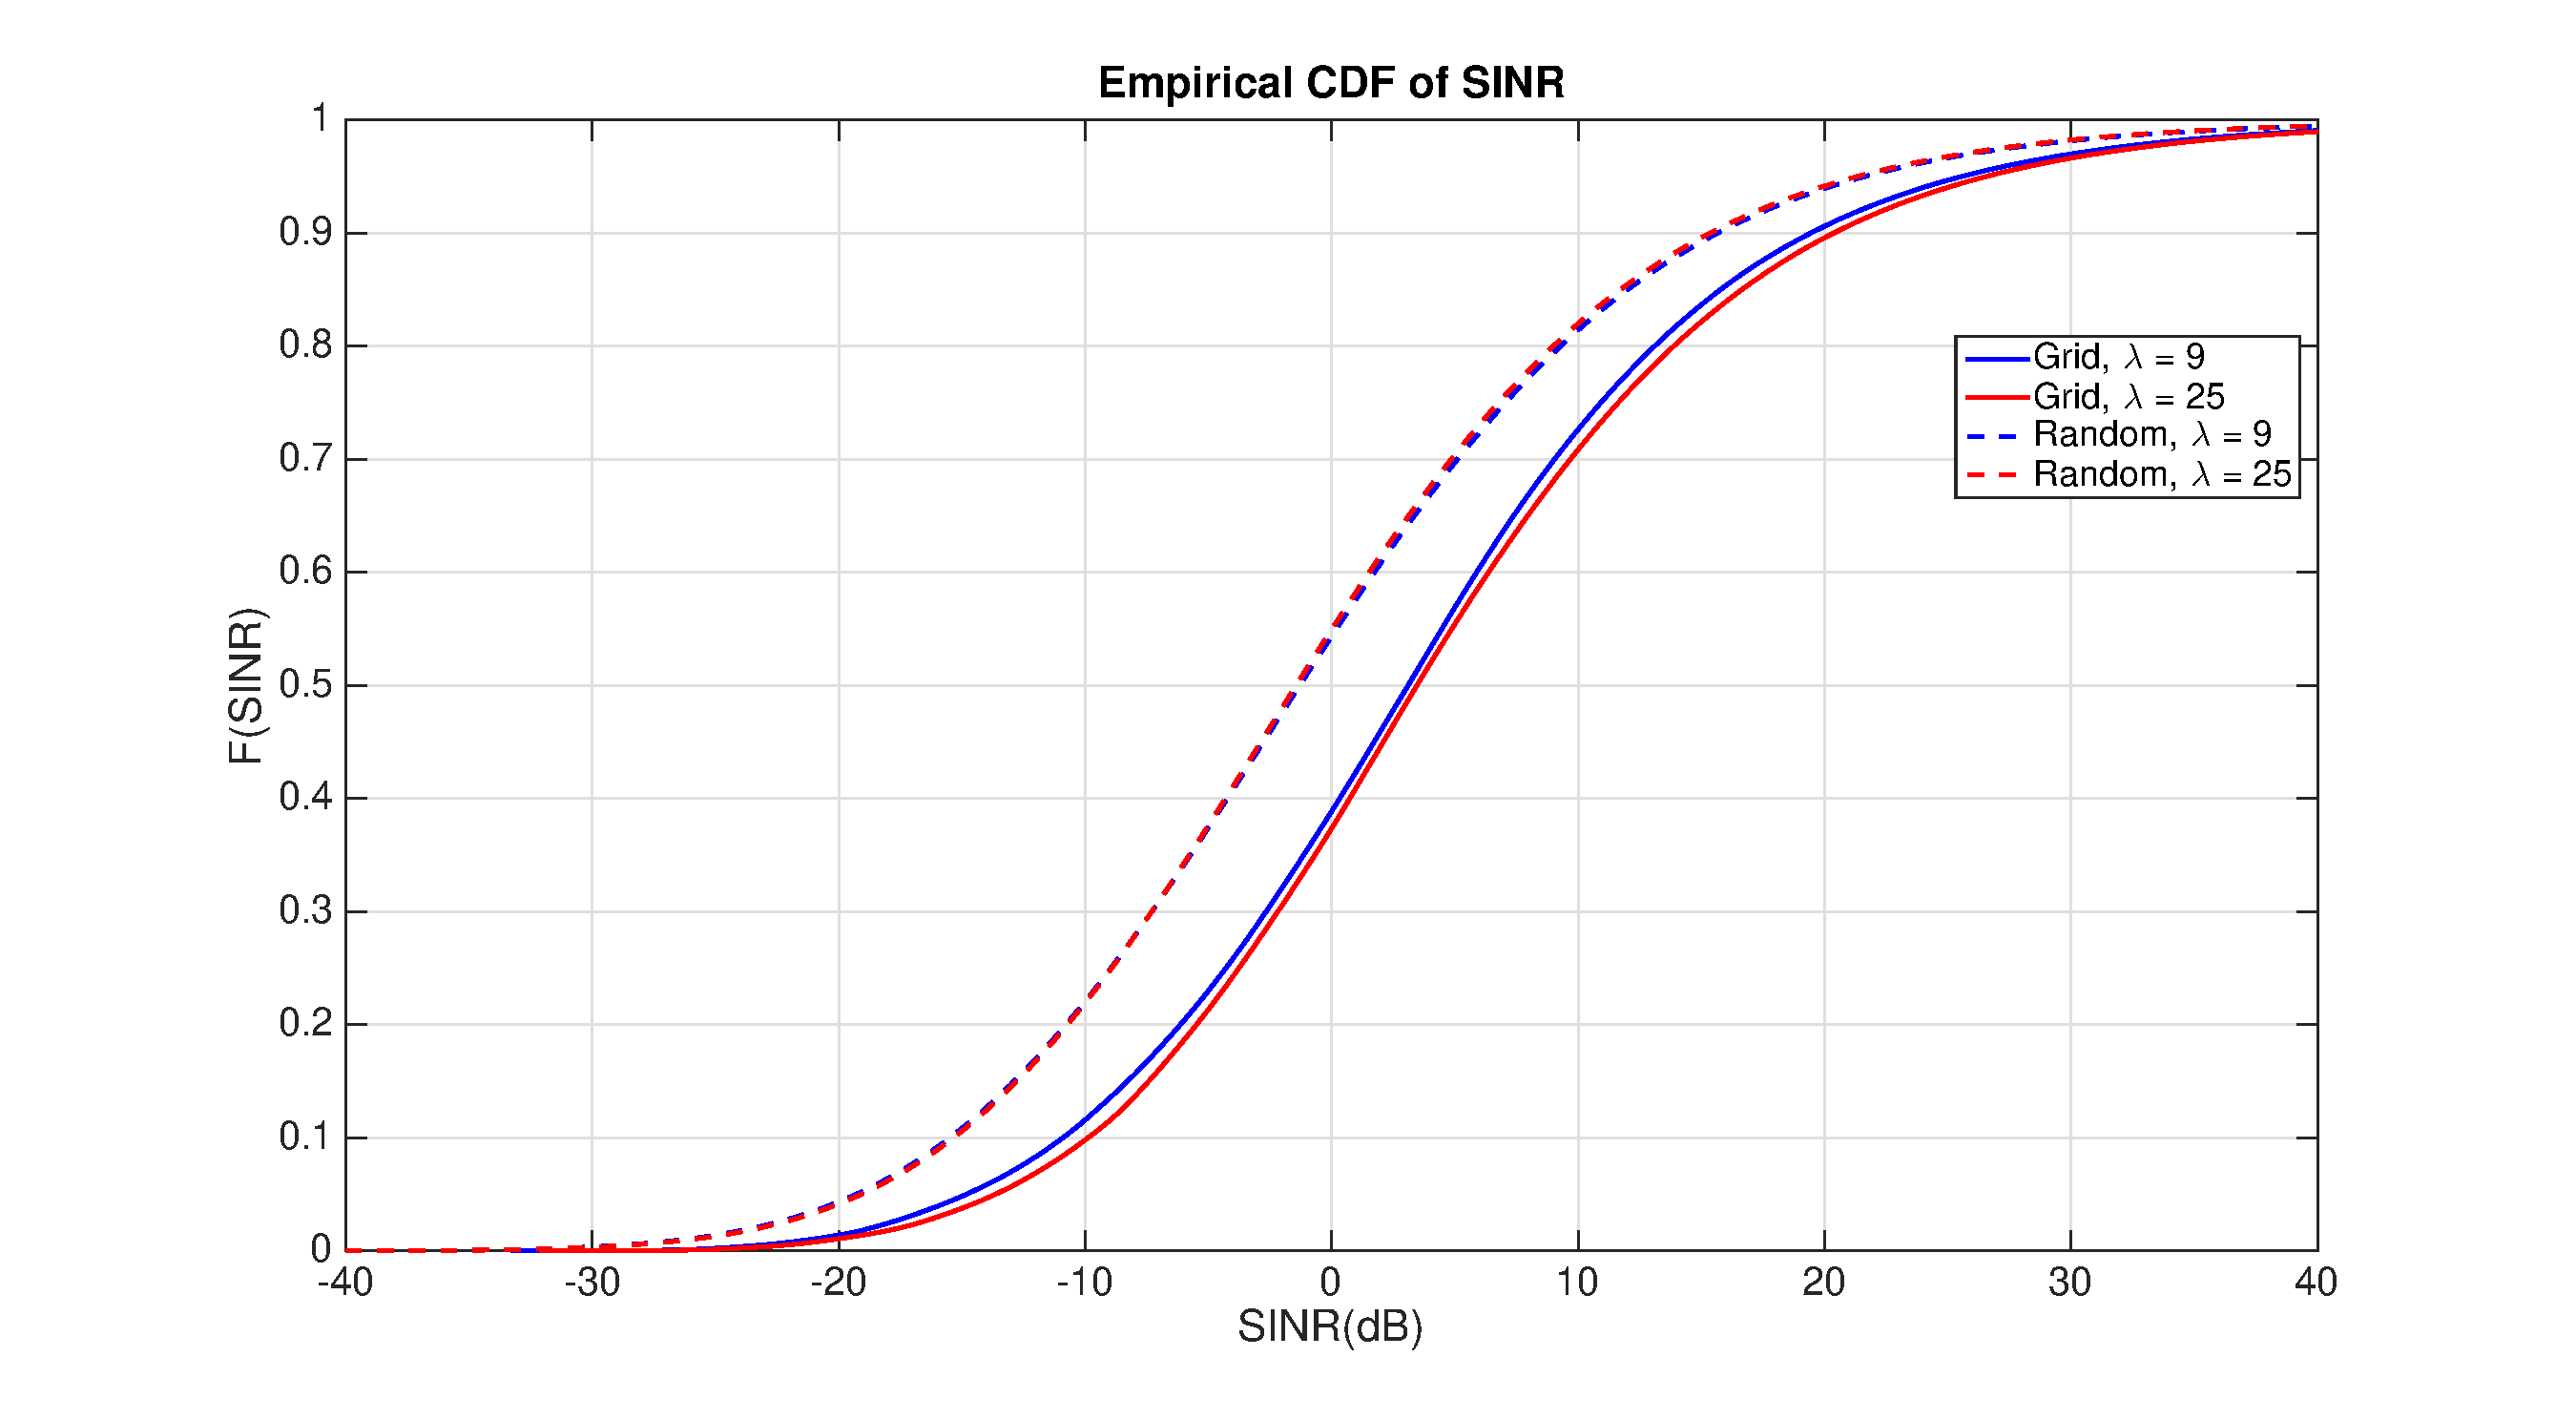
\includegraphics[width=14cm]{GridVSRandom.eps}
\caption{CDF of SINR given Grid Layout and Random Layout (De-Correlation Distance: $20m$)}
\label{cdf1}
\end{figure}
\begin{figure}
\centering
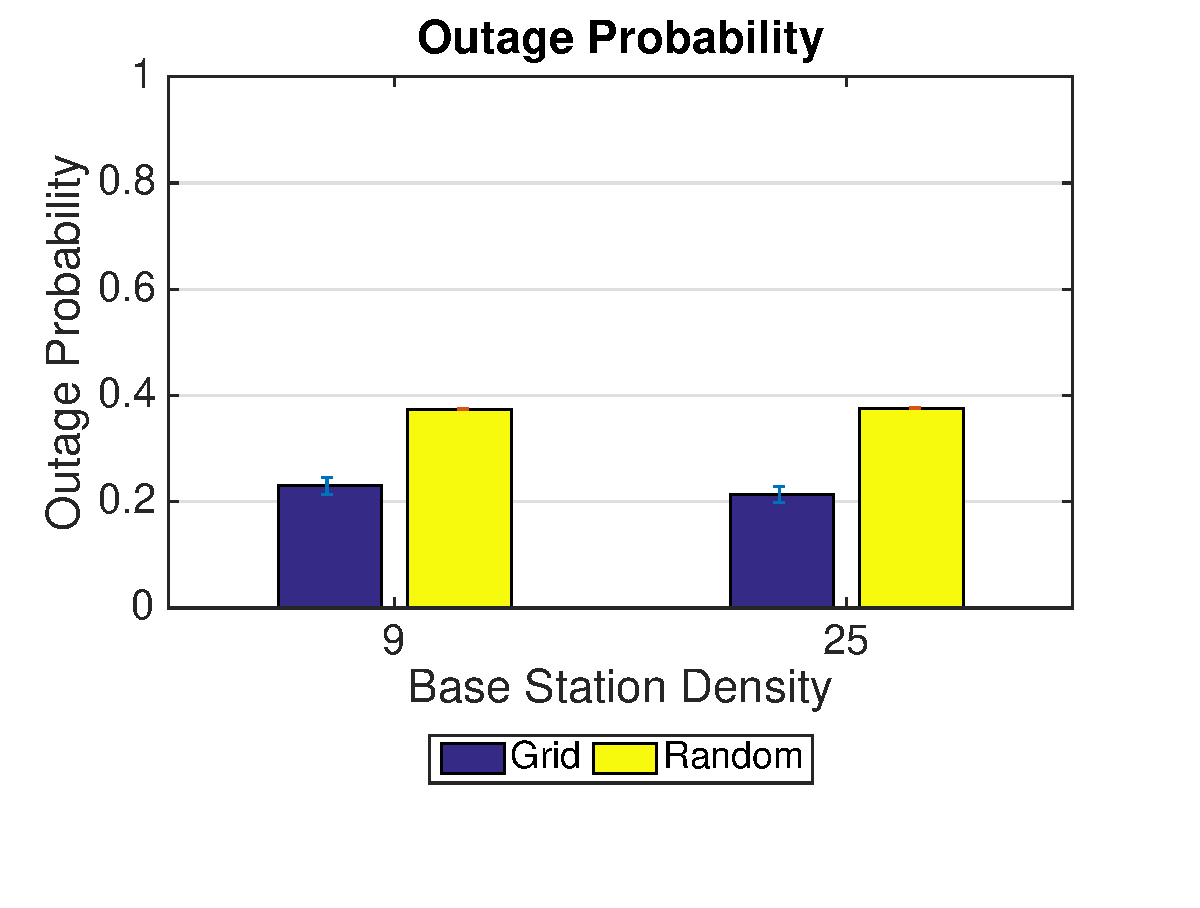
\includegraphics[width=14cm]{OutageProbGridVSRandom.eps}
\caption{Outage Probability given Grid Layout and Random Layout (De-Correlation Distance: $20m$)}
\label{outage1}
\end{figure}
\par For Random Layout, SINR distribution and outage probability of different BS densities are investigated for both nearest BS connection and best channel BS connection. 

